% Email: pbaeyens31+github@gmail.com
% Licencia: CC BY-SA 3.0

%% Paquetes y configuración %

% Beamer
\PassOptionsToPackage{unicode}{hyperref}  % Evita errores con caracteres no ASCII
\PassOptionsToPackage{naturalnames}{hyperref} % tex.stackexchange.com/questions/10555
\documentclass[compress]{beamer}
\usepackage{adjustbox}
% Idioma
\usepackage[spanish]{babel} % Traducciones
\usepackage[utf8]{inputenc} % Uso de caracteres UTF-8
\usepackage{lmodern}        % Fuentes de tamaño arbitrario
\usepackage[T1]{fontenc}    % Permite copiar y evita errores
%\uselanguage{Spanish}       % Traducciones beamer
%\languagepath{Spanish}      % (tex.stackexchange.com/questions/168208)

\usepackage{multicol}
\usepackage{multirow}

% Matemáticas
\usepackage{amsfonts}
\usepackage{amsmath}
\usepackage{amssymb}
\usepackage{marginnote}
% Colores
\definecolor{backg}{HTML}{F2F2F2}    % Fondo
\definecolor{title}{HTML}{bdc3d1}    % Títulos
\definecolor{comments}{HTML}{BDBDBD} % Comentarios
\definecolor{keywords}{HTML}{08388c} % Palabras clave
\definecolor{strings}{HTML}{FA5858}  % Strings
\definecolor{links}{HTML}{2C2C95}    % Enlaces
\definecolor{bars}{HTML}{045FB4}     % Barras (gráfico)

% Código
\usepackage{listings}
\lstset{
language=[LaTeX]TeX,
basicstyle=\footnotesize,
morekeywords={href,uselanguage,languagepath,column},
otherkeywords={pause,usetheme,usecolortheme,useinnertheme,titlepage,tableofcontents,subtitle},
breaklines=true,
backgroundcolor=\color{backg},
keywordstyle=\color{keywords},
commentstyle=\color{comments},
stringstyle=\color{strings},
tabsize=2,
% Acentos, ñ, ¿, ¡ (tex.stackexchange.com/questions/24528)
extendedchars=true,
literate={á}{{\'a}}1 {é}{{\'e}}1 {í}{{\'i}}1 {ó}{{\'o}}1
         {ú}{{\'u}}1 {ñ}{{\~n}}1 {¡}{{\textexclamdown}}1
         {¿}{{?`}}1
}

% Gráficos
\usepackage{pgfplots}
\pgfplotsset{width=7cm,compat=1.14} % Opciones para gráficos

% Emoticonos
\usepackage{wasysym}
\usepackage{graphicx}
% tikz
\usepackage{tikz}
\usetikzlibrary{mindmap,trees,shadows}
\tikzset{ % Genera overlays
    invisible/.style={opacity=0},
    visible on/.style={alt={#1{}{invisible}}},
    alt/.code args={<#1>#2#3}{\alt<#1>{\pgfkeysalso{#2}}{\pgfkeysalso{#3}}},
}

%% Comandos %%
\newcommand{\ejemplo}[1]{\lstinputlisting{./examples/#1}} % Mostrar código de ejemplos
\newcommand{\muestra}[1]{\input{./examples/#1}}           % Mostrar ejemplos
\newcommand{\seccion}[1]{\input{./sections/#1}}           % Incluir secciones
\newcommand{\espacio}{\vspace*{\baselineskip}}            % Añade espacios
\newcommand{\beamer}{\texttt{beamer} }                    % Estilo único para beamer
\newcommand{\enlace}[3]{\href{#1}{\textbf{#2}} - {\small #3}}  % Estílo único para refs
\newcommand{\comando}[1]{{\color{black}\textbackslash}{\color{keywords}#1}}
\newcommand{\marginalnote}[1]{\mbox{}\marginpar{\raggedright\hspace{0pt}#1}}
%% Temas %%
% Tema y tema de color
  \usetheme{Dresden}
  \usecolortheme{dolphin}
  \useinnertheme{circles}
  \setbeamercovered{transparent}
% Colores bloques
  \setbeamercolor{block title}{bg=title,fg=links}
  \setbeamercolor{block body}{bg=backg,fg=black}
  \setbeamercolor{block title alerted}{fg=red!70!black,bg=title!92!red}
  \setbeamercolor{block body alerted}{fg=black,bg=backg}
  \setbeamercolor{block title example}{fg=green!70!black,bg=title!92!green}
  \setbeamercolor{block body example}{fg=black,bg=backg}
% Enlaces (tex.stackexchange.com/questions/13423)
\hypersetup{colorlinks,linkcolor=,urlcolor=links}
% Quita enlaces de navegación (stackoverflow.com/questions/3017030)
\setbeamertemplate{navigation symbols}{}
% Quita barra inferior (stackoverflow.com/questions/1435837)
\setbeamertemplate{footline}{}
% Evita warnings boxes
\hfuzz=20pt
\vfuzz=20pt
% Evita wranings itemize
\renewcommand\textbullet{\ensuremath{\bullet}}

%% Título y otros %%
\title{Práctica 2}                                               % Título
\subtitle{Divide y vencerás}                                  % Subtítulo
\author{Laura Gómez Garrido, Pedro Bonilla Nadal, Javier Sáez Maldonado, Daniel Pozo Escalona, Luis Ortega Andrés}

\date{2º Doble Grado Informática y Matemáticas}                                                            % Fecha

%% Listing settings

\usepackage{color}

\definecolor{dkgreen}{rgb}{0,0.6,0}
\definecolor{gray}{rgb}{0.5,0.5,0.5}
\definecolor{mauve}{rgb}{0.58,0,0.82}

\lstset{frame=tb,
  language=Java,
  aboveskip=3mm,
  belowskip=3mm,
  showstringspaces=false,
  columns=flexible,
  basicstyle={\small\ttfamily},
  numbers=none,
  numberstyle=\tiny\color{gray},
  keywordstyle=\color{blue},
  commentstyle=\color{dkgreen},
  stringstyle=\color{mauve},
  breaklines=true,
  breakatwhitespace=true,
  tabsize=3
}

%% Presentación %%
\begin{document}

\begin{frame}
\titlepage
\end{frame}

\begin{frame}{Índice}
  \hypertarget{index}{}
  \tableofcontents
  
\end{frame}

\section{Problema}
\begin{frame}

\textbf{\\Problema 6.\\}
		Sea un vector $v$ de números de tamaño $n$, todos distintos, de forma que existe un índice $p$ (que no es ni el primero ni el último) tal que a la izquierda de $p$ los números están ordenados de forma creciente y a la derecha de $p$ están ordenados de forma decreciente; es decir%\\
%\hfill\\
$$\forall \ i,j \leq p , \ i < j \rightarrow v[i] < v[j] \quad y \quad \forall \ i,j \geq p, \ i < j \rightarrow v[i]>v[j]$$\\
%\hfill\\
(de forma que el máximo se encuentra en la posición $p$). Diseñe un algoritmo ``divide y vencerás'' que permita determinar $p$. ¿Cuál es la complejidad del algoritmo? Compárelo con el algoritmo ``obvio'' para realizar esta tarea. Realizar también un estudio empírico e híbrido de la eficiencia de ambos algoritmos.

\end{frame}	
	
\section{Solución}

\subsection{El algoritmo obvio}

\begin{frame}
	Para empezar buscamos un algoritmo obvio que utilice la fuerza bruta para buscar la solución. En este algoritmo hacemos una búsqueda lineal del punto donde empiece a decrecer el vector.
\end{frame}

\begin{frame}[fragile]
	\frametitle{Código fuerza bruta}
 \begin{lstlisting}
 int fuerzaBruta(int* v, int n){
   for(int i=1; i < n-1; ++i){
     if(v[i] > v[i+1])
       return i;
   }
 }
 \end{lstlisting}
\end{frame}

\subsection{Divide y vencerás}
\begin{frame}
        Utilizamos ahora la estrategia divide y vencerás para crear un algoritmo
de orden logarítmico.\\
	%Sabemos que nuestro método utiliza la técnica divide y vencerás pues lo que estamos haciendo es dividir el vector en mitades de forma sucesiva. El algoritmo consiste en ir mirando en la mitad del vector (sea esta mitad la posición p) y comparando si los elementos en las posiciones p − 1, p y p + 1 están en orden ascendente, y en cuyo caso realizar de nuevo esta operación sobre el vector que queda a la izquierda de esta posición, o si están en orden descendente, y entonces realizar esta operación sobre el vector que queda a la derecha de esta posición.

\end{frame}
\newlength\someheight
\setlength\someheight{3.5cm}

\begin{frame}[fragile]
\frametitle{Código divide y vencerás}
\begin{center}
 \begin{adjustbox}{width=\textwidth,height=\someheight,keepaspectratio}
 	\begin{lstlisting}
 	int divideYVenceras(int* v, int n){
 	int k = n/2;
 	if(n==1)
	 	return 0; //Caso trivial
 	
 	if(n==2)
	 	 return v[0]>v[1]?0:1; //Entre dos elementos, manda el más grande.
 	
	 if(v[k] > v[k+1]){

 		if(v[k] > v[k-1]) 
	 		return k;
 		
	 	//else
 		return divideYVenceras(v,k);
 	}
 		
 	//else
 	return k + 1 + divideYVenceras(v+k+1,n-k-1);
 	}
 		\end{lstlisting}
 		\end{adjustbox}
 		\end{center}
 		
\end{frame}

\begin{frame}[fragile]
  \frametitle{El funcionamiento de la solución}
  \begin{lstlisting}
   if(v[k] > v[k+1]){
     if(v[k] > v[k-1]) 
       return k;
     return divideYVenceras(v,k);
   }
   return k + 1 + divideYVenceras(v+k+1,n-k-1);
\end{lstlisting}

\begin{center}
  \begin{tabular}{|l|l|l|l|l|l|l|l|l|l|}
\hline
1 & 2 & 3 & 4 & 5 & 6 & 10 & 9 & 8 & 7 \\ \hline
\end{tabular}
\end{center}
\end{frame}



\subsection{Resultados empíricos}
\begin{frame}
	Ahora expondremos los resultados de la ejecución de ambos códigos:\\
	\begin{center}
	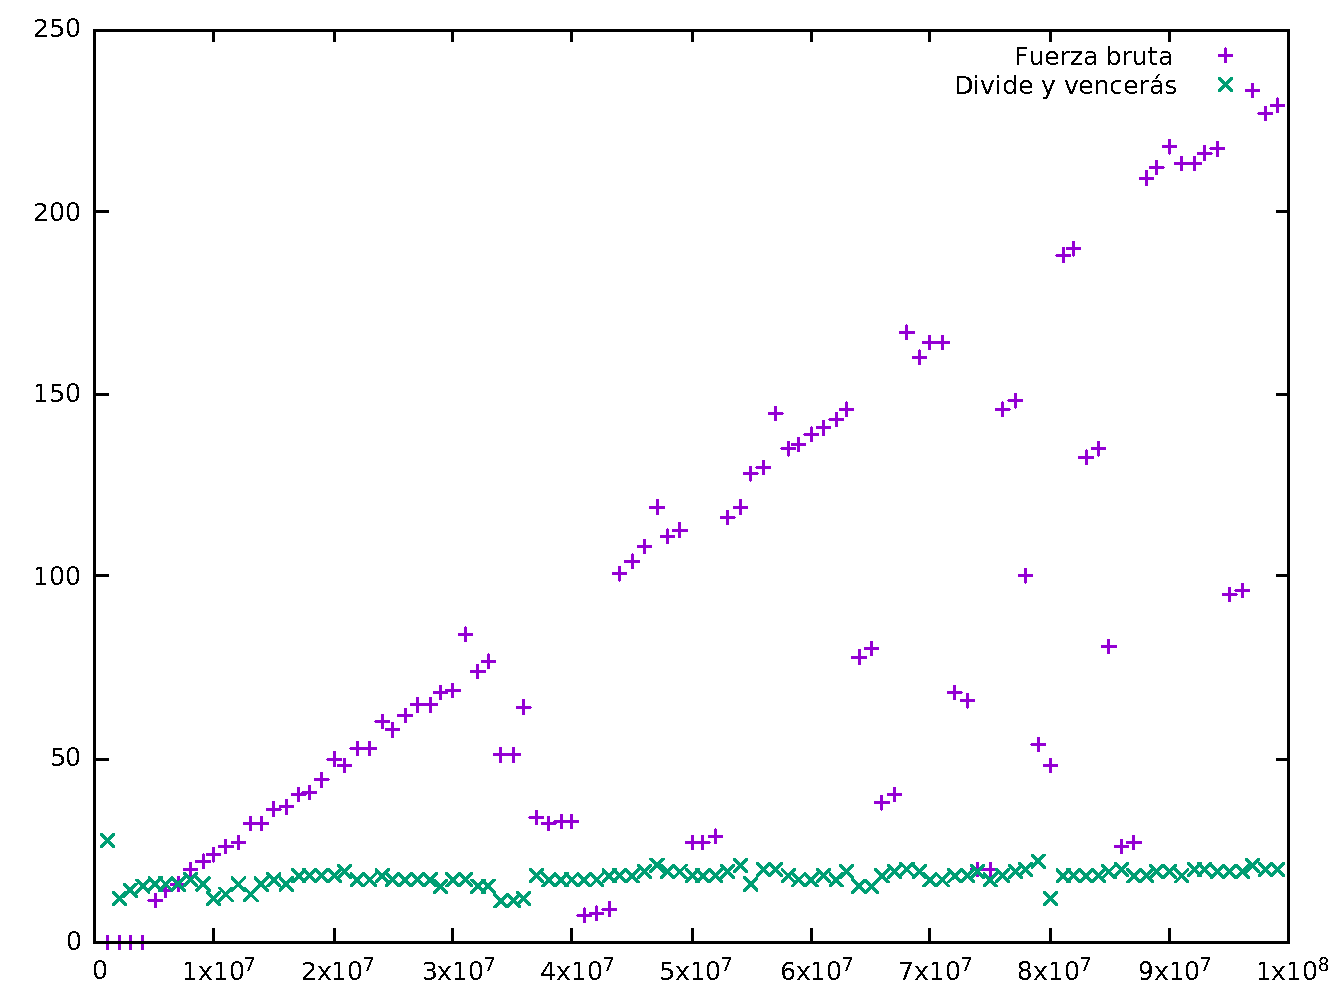
\includegraphics[scale=0.37]{imagen1.pdf}
\end{center}
\end{frame}
	
\begin{frame}
\frametitle{Coeficientes de los ajustes de las curvas}
Por ultimo vamos a ajustar por mínimos cuadrados cada una de las gráficas de acuerdo con la curva obtenida en el análisis teórico para hallar la eficiencia híbrida.

\begin{block}{Curva parametrizada para divide y vencerás}
	$a\log(x)+b$
\end{block}

\begin{block}{Curva parametrizada para fuerza bruta}
	$ax+b$
\end{block}
\end{frame}

\begin{frame}
	\begin{center}
	\begin{tabular}{ll}
	Algoritmo & Coeficientes\\ \hline\noalign{\smallskip}
	\textit{Divide y vencerás} & $\begin{array}{ll}
	a = 0.754033 \\
b = 4.34225 
\end{array}$ \\\hline\noalign{\smallskip}
	\textit{Fuerza bruta} & $\begin{array}{ll}
	a = 1.64383e-06 \\
b = 4.33354

\end{array}$ \\\hline\noalign{\smallskip}
\end{tabular}
\end{center}
\end{frame}

\begin{frame}
  \frametitle{Ajuste de los datos}
  \begin{center}
  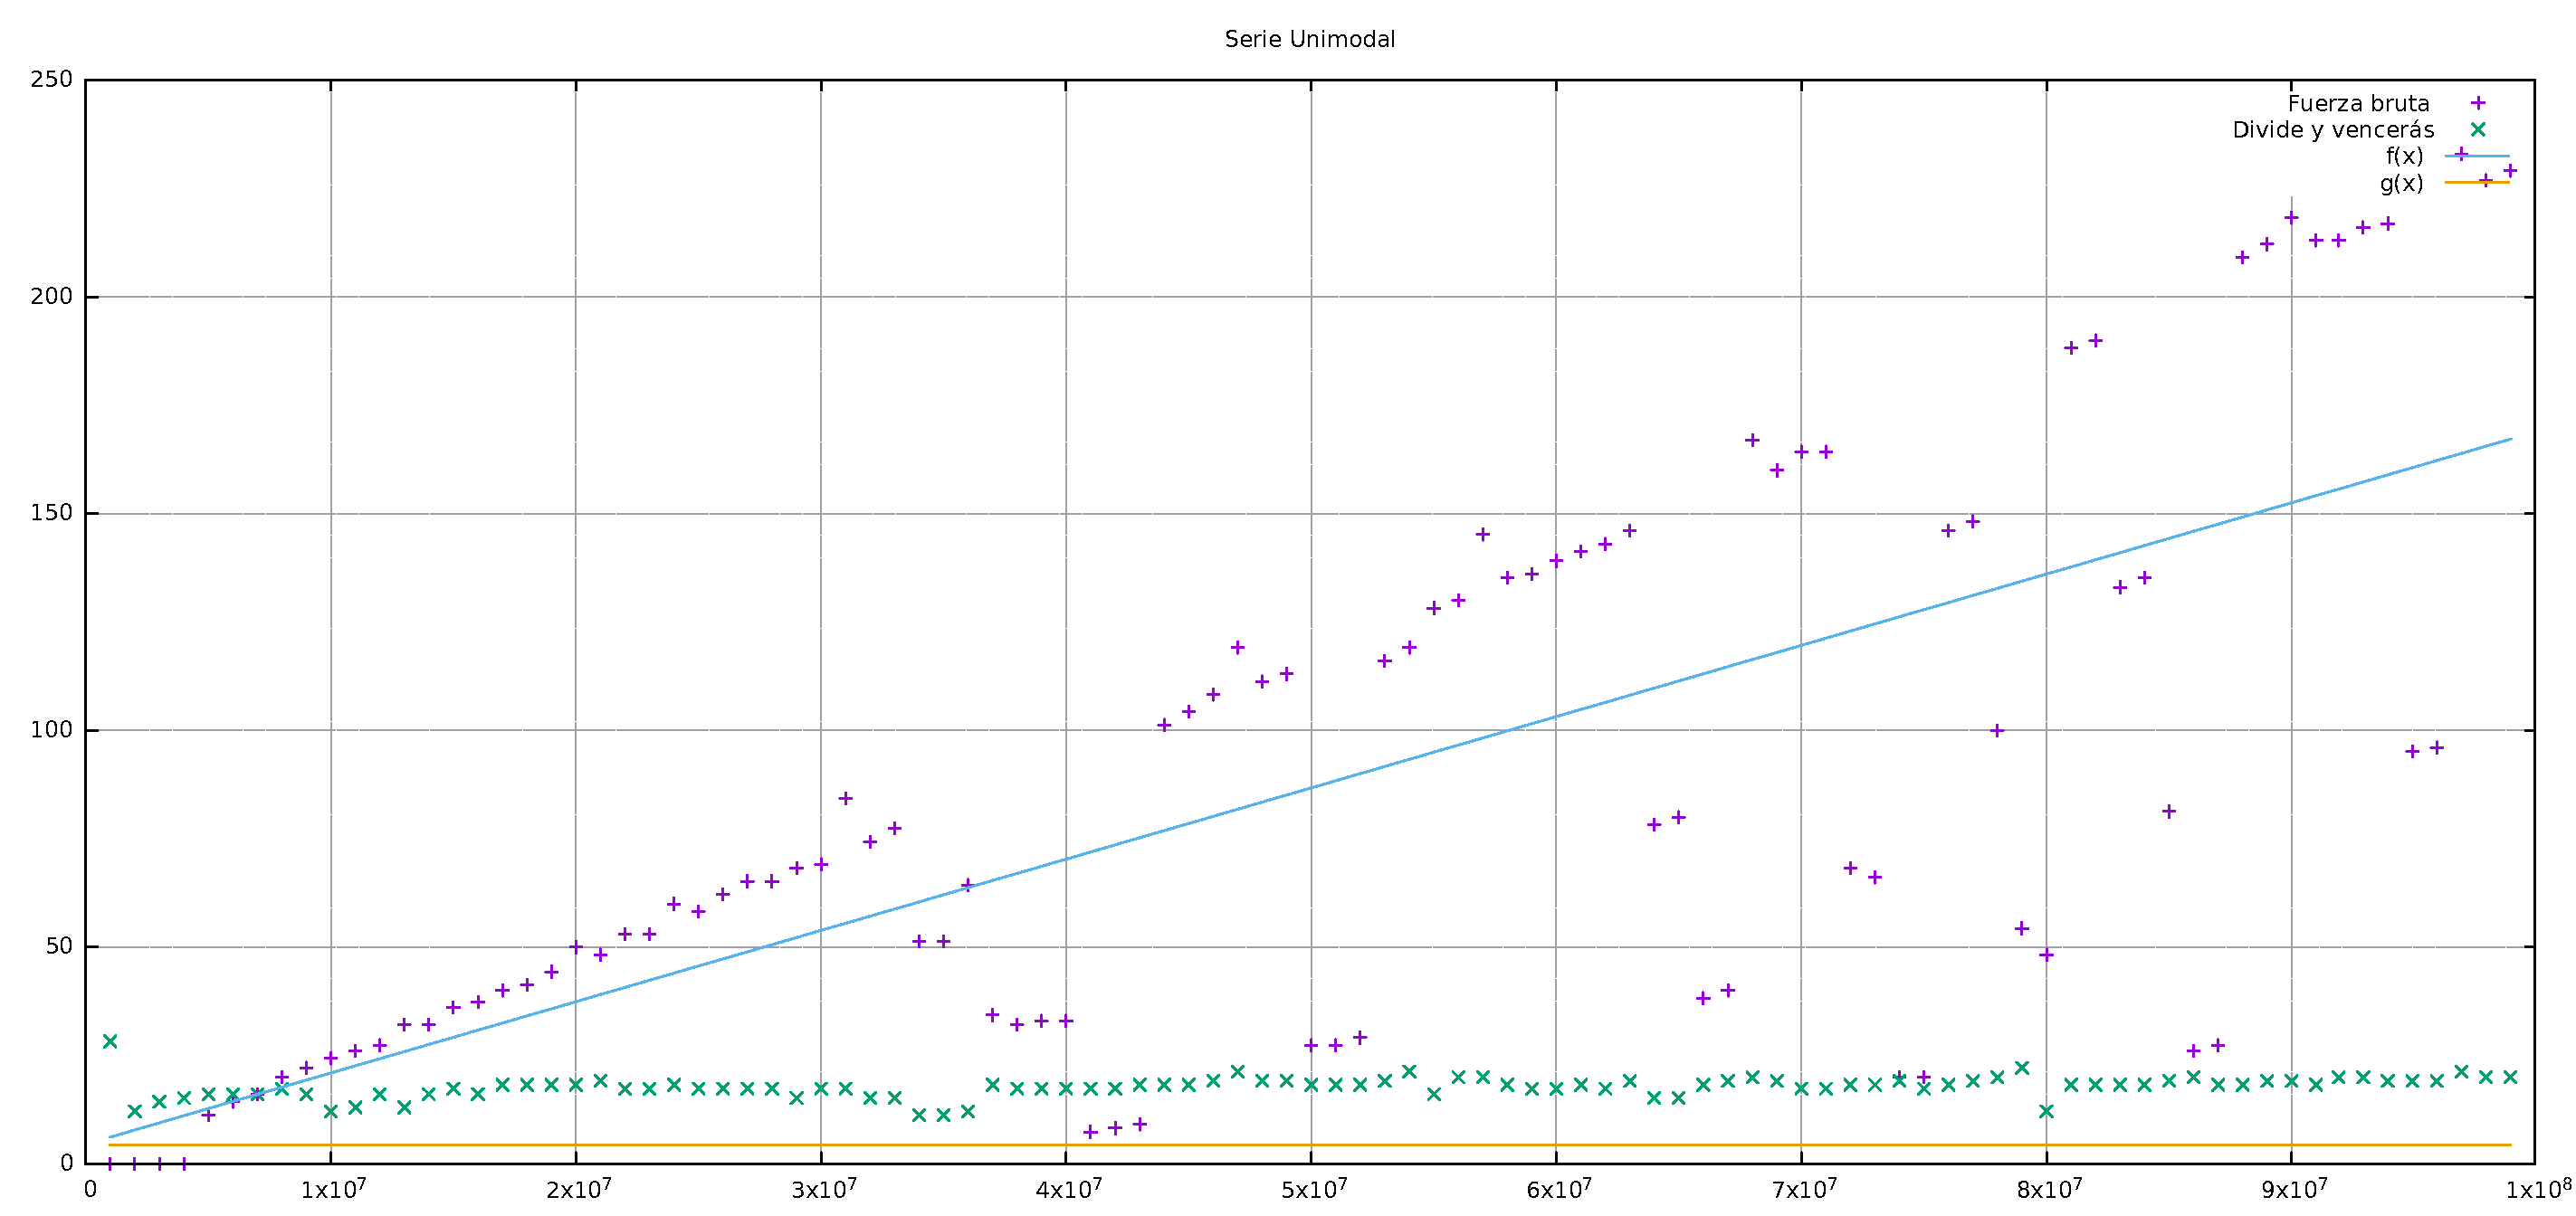
\includegraphics[scale=0.23]{ajuste.pdf}
\end{center}
\end{frame}
\end{document}
